\documentclass[referee, pdflatex, sn-mathphys-num]{sn-jnl}

\usepackage{hyperref}
\usepackage{geometry} 
\usepackage{subfigure}
\usepackage{graphicx} 
\usepackage{amsmath,amsfonts,amssymb,amsthm,mathtools}
\usepackage{icomma}
\usepackage[english]{babel}
\usepackage{array,tabularx,tabulary,booktabs}
\usepackage{multirow}
\usepackage{diagbox}

\theoremstyle{definition}
\newtheorem{Def}{Definition}
\theoremstyle{plain}
\newtheorem{Lem}{Lemma}
\newtheorem{Th}{Theorem}

\begin{document}
	
	\title{Time series classification in parameters space using NeuralODE}
	
	\author*[1]{\fnm{Kirill} \sur{Semkin}}\email{semkin.ki32@gmail.com}
	\author*[2]{\fnm{Vadim} \sur{Strijov}}\email{strijov@forecsys.ru}
	
	%\affil*[1]{\orgname{Forecsys LLC} \orgaddress{\city{Moscow}} \country{Russia}}
	%\affil*[2]{\orgname{Forecsys LLC} \orgaddress{\city{Moscow}} \country{Russia}}
	
	\keywords{time series; NeuralODE; classification; inertial measurement unit}
	
	\maketitle
	
	\begin{abstract}
		
		The task of time series classification is to assign class label to given time series. The number of classes is fixed. It is assumed that each class corresponds to some dynamical system. Each system generates phase trajectories within some probabilistic model. These trajectories are then mapped into empirical observations. The paper investigates how to restore dynamical systems out of experimental data using NeuralODE. We consider fixed and bayesian approaches to defining dynamical systems' parameters. Two classification principles are introduced: bayesian testing and transition to dynamical system's parameters space. Taken's theorem is used to approximate true phase trajectories. At last, time series from inertial measurement unit are classified using given technics and compared with other machine learning models.
		
	\end{abstract}
	
	\section{Introduction}\label{Intro}
	
	Current theory is not well established yet. Here are basic ideas and schemes of the probabilistic frameworks used in the work.
	
	\begin{figure}[h]
		\centering
		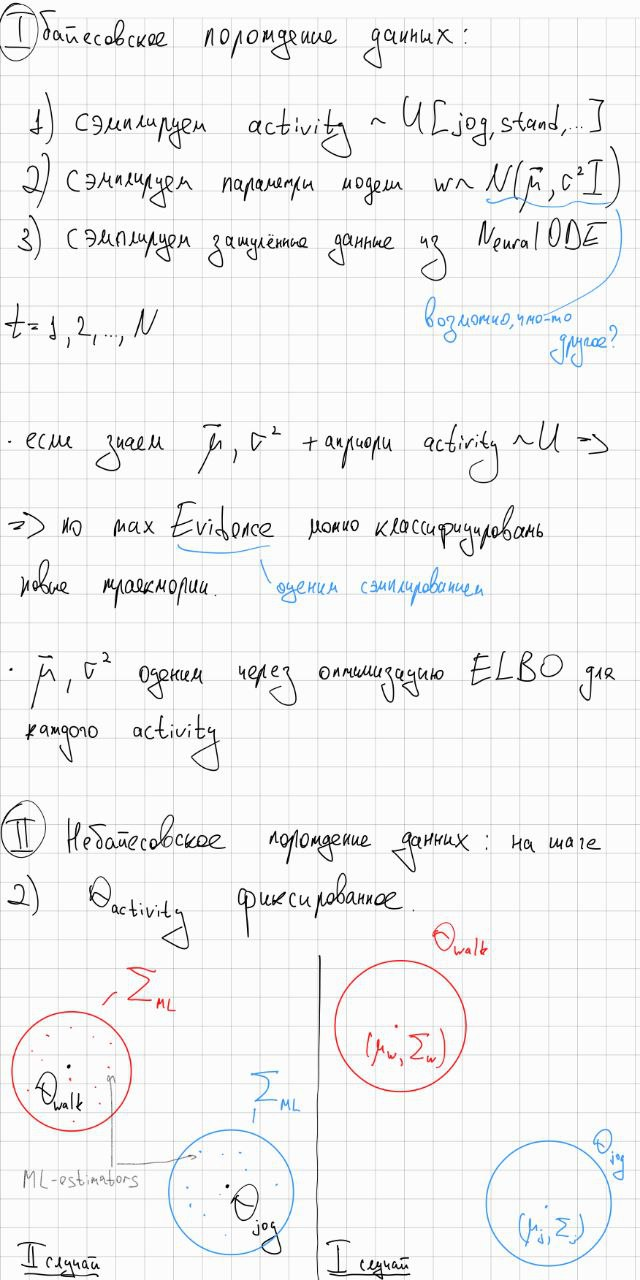
\includegraphics[width=0.8\textwidth]{imgs/photo_1_2024-12-13_23-46-45}
	\end{figure}
	
	\begin{figure}[h]
		\centering
		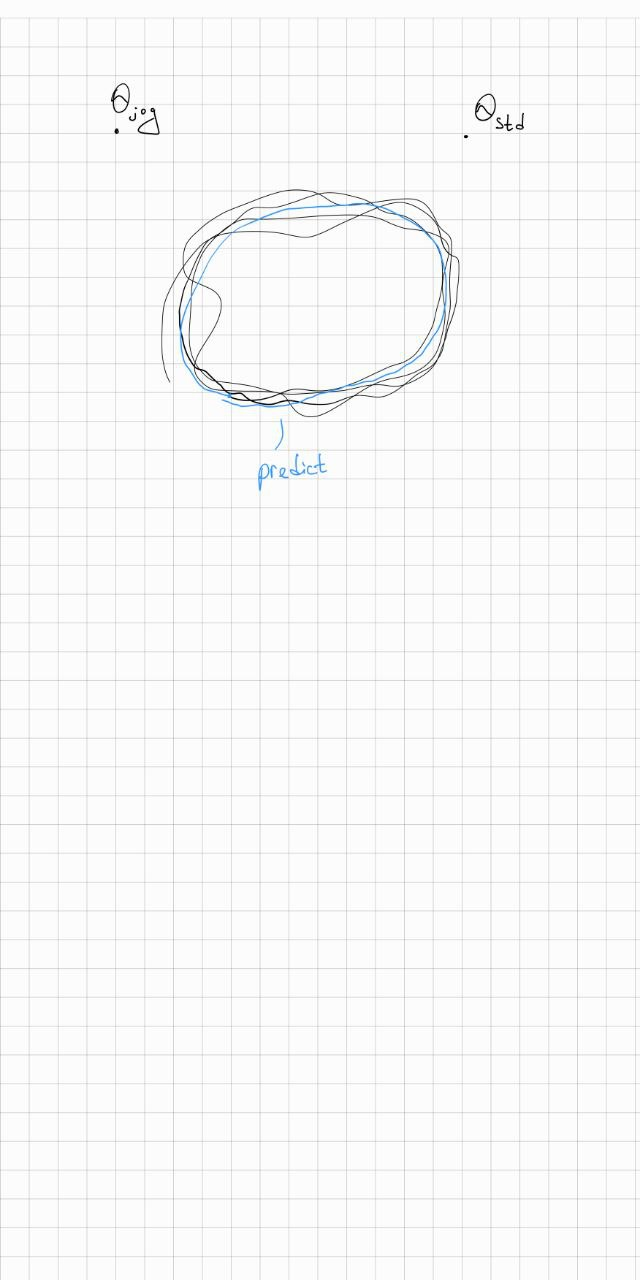
\includegraphics[width=0.8\textwidth]{imgs/photo_2_2024-12-13_23-46-45}
	\end{figure}
	
	\begin{figure}[h]
		\centering
		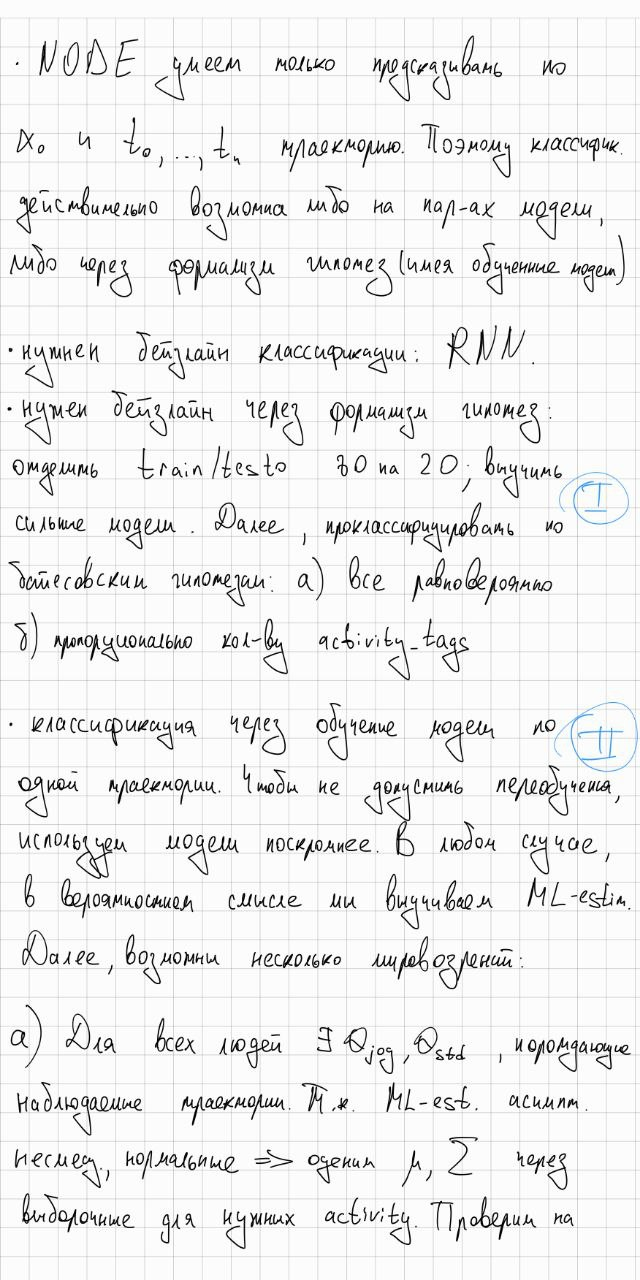
\includegraphics[width=0.8\textwidth]{imgs/photo_3_2024-12-13_23-46-45}
	\end{figure}
	
	\begin{figure}[h]
		\centering
		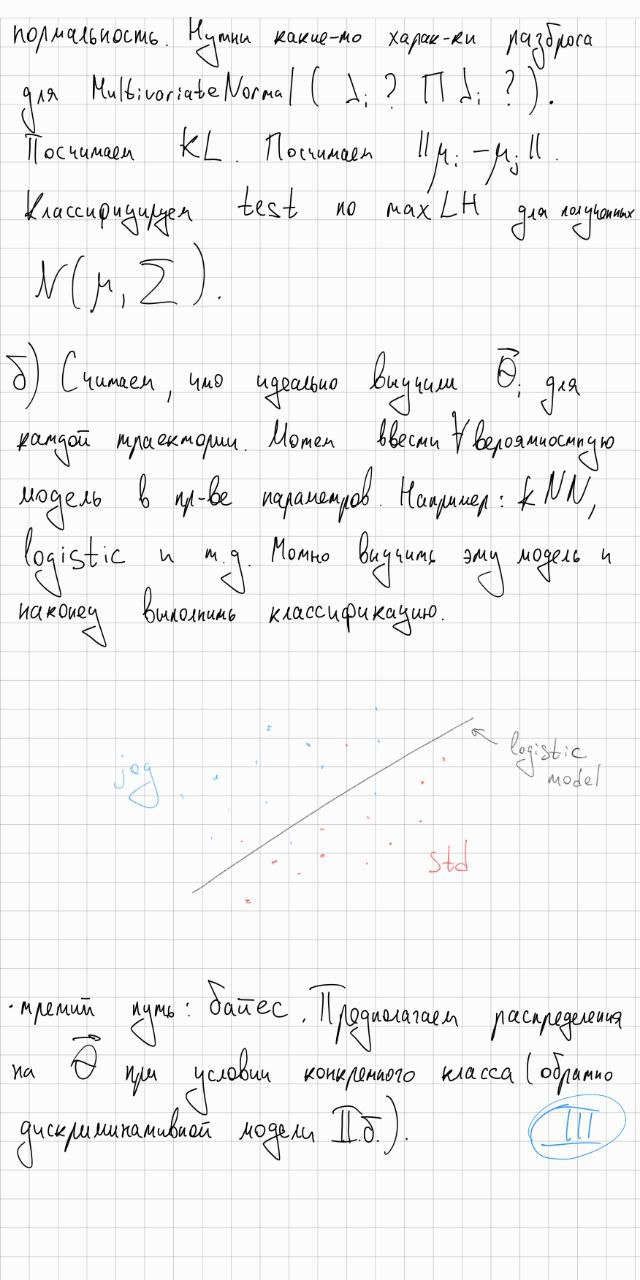
\includegraphics[width=0.8\textwidth]{imgs/photo_4_2024-12-13_23-46-45}
	\end{figure}
	
	
	
 \end{document}